\documentclass[11pt,a4paper,oneside]{book}
%-- coding: UTF-8 --
\usepackage[UTF8]{ctex}
\usepackage{fontspec}
\defaultfontfeatures{Mapping=tex-text}
\usepackage{xunicode}%防止pdf乱码
%\usepackage{ccmap}%
\usepackage{xltxtra}
\usepackage{amsmath}
\usepackage{amsfonts}
\usepackage{amssymb}
\usepackage{graphicx}
\usepackage{amsthm}
\usepackage{array}
\usepackage{float}   %{H}
\usepackage{booktabs}  %\toprule[1.5pt]
\setcounter{secnumdepth}{4}
\usepackage{indentfirst} %首行缩进
\usepackage{tcolorbox} %彩色框框
\usepackage{graphicx}  %图片并排
\usepackage{subfigure} %图片并排
\usepackage{graphicx} %插入jpg
\usepackage[toc]{multitoc}
\setcounter{secnumdepth}{4}		%增加编号深度
\setcounter{tocdepth}{4}		%增加目录深度
\usepackage{hyperref}     %生成pdf书签
\hypersetup{hidelinks,
	colorlinks=true,
	allcolors=black,
	pdfstartview=Fit,
	breaklinks=true
}       %去掉目录的红色框框
%===================%插入代码需要的控制
\usepackage{listings}
\usepackage{xcolor}
\setmonofont{Consolas}%字体
\definecolor{grey}{rgb}{0.8,0.8,0.8}
\definecolor{darkgreen}{rgb}{0,0.3,0}
\definecolor{darkblue}{rgb}{0,0,0.3}
\def\lstbasicfont{\fontfamily{pcr}\selectfont\footnotesize}
\lstset{%
	numbers=left,
	numberstyle=\tt\tiny,%
	showstringspaces=false,
	showspaces=false,%
	tabsize=4,%
	frame=lines,%
	basicstyle=\tt\small,%
	keywordstyle=\color{ blue!70}\bfseries,%
	identifierstyle=,%
	commentstyle=\color{red!50!green!50!blue!50},%\itshape,%
	stringstyle=\color{black},%
	breaklines=true
}
%===================%
\usepackage[left=2cm,right=2cm,top=2cm,bottom=2cm]{geometry}
\newtheorem{theorem}{定理}
\newtheorem{definition}{定义}
\newtheorem{e}{例}
\title{\Huge NOTE on R}
\author{zy}
\date{\today}

\begin{document}
\maketitle
\tableofcontents  %目录
\chapter{创建数据集}
\section{数据集的定义}

不同的行业对于数据集的行和列叫法不同。统计学家称它们为观测(observation)和变量(variable),数据库分析师则称其为记录(record)和字段(field),数据挖掘/机器学习学科的研究者则把它们叫做示例(example)和属性(attribute)。我们在本书中通篇使用术语观测和变量。

\section{数据结构}
\subsection{向量}

向量是用于存储数值型、字符型或逻辑型数据的一维数组。执行组合功能的函数c()可用来创建向量.

\begin{lstlisting}[language=R]
> data("iris")
> iris <- data.frame(iris)

> sl <- iris$Sepal.Length
> sl
[1] 5.1 4.9 4.7 4.6 5.0 5.4 4.6 5.0 4.4 4.9 5.4 4.8 4.8 4.3
[15] 5.8 5.7 5.4 5.1 5.7 5.1 5.4 5.1 4.6 5.1 4.8 5.0 5.0 5.2
[29] 5.2 4.7 4.8 5.4 5.2 5.5 4.9 5.0 5.5 4.9 4.4 5.1 5.0 4.5
[43] 4.4 5.0 5.1 4.8 5.1 4.6 5.3 5.0 7.0 6.4 6.9 5.5 6.5 5.7
[57] 6.3 4.9 6.6 5.2 5.0 5.9 6.0 6.1 5.6 6.7 5.6 5.8 6.2 5.6
[71] 5.9 6.1 6.3 6.1 6.4 6.6 6.8 6.7 6.0 5.7 5.5 5.5 5.8 6.0
[85] 5.4 6.0 6.7 6.3 5.6 5.5 5.5 6.1 5.8 5.0 5.6 5.7 5.7 6.2
[99] 5.1 5.7 6.3 5.8 7.1 6.3 6.5 7.6 4.9 7.3 6.7 7.2 6.5 6.4
[113] 6.8 5.7 5.8 6.4 6.5 7.7 7.7 6.0 6.9 5.6 7.7 6.3 6.7 7.2
[127] 6.2 6.1 6.4 7.2 7.4 7.9 6.4 6.3 6.1 7.7 6.3 6.4 6.0 6.9
[141] 6.7 6.9 5.8 6.8 6.7 6.7 6.3 6.5 6.2 5.9

> summary(sl)
 Min. 1st Qu.  Median    Mean 3rd Qu.    Max. 
4.300   5.100   5.800   5.843   6.400   7.900 
> str(sl)
num [1:150] 5.1 4.9 4.7 4.6 5 5.4 4.6 5 4.4 4.9 ...

> sl[4]
[1] 4.6
> sl[c(1,2,3)]
[1] 5.1 4.9 4.7
> sl[1:5]
[1] 5.1 4.9 4.7 4.6 5.0
\end{lstlisting}

\subsection{矩阵}

\begin{lstlisting}[language=R]
> i1 <- iris[1:4,1:4]
> i1 <- as.matrix(i1)
> i1
  Sepal.Length Sepal.Width Petal.Length Petal.Width
1          5.1         3.5          1.4         0.2
2          4.9         3.0          1.4         0.2
3          4.7         3.2          1.3         0.2
4          4.6         3.1          1.5         0.2

> i1 <- as.vector(i1)
> i1
[1] 5.1 4.9 4.7 4.6 3.5 3.0 3.2 3.1 1.4 1.4 1.3 1.5 0.2 0.2
[15] 0.2 0.2
> i2 <- matrix(i1,nrow = 4,ncol = 4,byrow = T,dimnames = list(c("a1","a2","a3","a4"),c("b1","b2","b3","b4")))
> i2
    b1  b2  b3  b4
a1 5.1 4.9 4.7 4.6
a2 3.5 3.0 3.2 3.1
a3 1.4 1.4 1.3 1.5
a4 0.2 0.2 0.2 0.2

> i2[1,]
b1  b2  b3  b4 
5.1 4.9 4.7 4.6 
> i2[1,4]
[1] 4.6
> i2[1,c(2,3)]
b2  b3 
4.9 4.7 
\end{lstlisting}

\subsection{数组}

数组(array)与矩阵类似,但是维度可以大于2.

\begin{lstlisting}[language=R]
> i3 <- array(iris$Sepal.Length[1:24],c(2,3,4))
> i3
, , 1

[,1] [,2] [,3]
[1,]  5.1  4.7  5.0
[2,]  4.9  4.6  5.4

, , 2

[,1] [,2] [,3]
[1,]  4.6  4.4  5.4
[2,]  5.0  4.9  4.8

, , 3

[,1] [,2] [,3]
[1,]  4.8  5.8  5.4
[2,]  4.3  5.7  5.1

, , 4

[,1] [,2] [,3]
[1,]  5.7  5.4  4.6
[2,]  5.1  5.1  5.1
\end{lstlisting}
\subsection{数据框}

\begin{figure}[H]
	\centering
	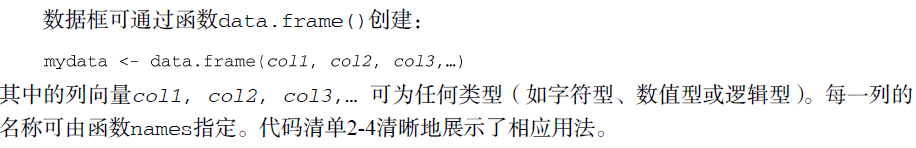
\includegraphics[width=\textwidth]{screenshot002}
	\label{fig:screenshot002}
\end{figure}

\begin{lstlisting}[language=R]
> head(iris)
  Sepal.Length Sepal.Width Petal.Length Petal.Width Species
1          5.1         3.5          1.4         0.2  setosa
2          4.9         3.0          1.4         0.2  setosa
3          4.7         3.2          1.3         0.2  setosa
4          4.6         3.1          1.5         0.2  setosa
5          5.0         3.6          1.4         0.2  setosa
6          5.4         3.9          1.7         0.4  setosa

> head(iris[1:2])
  Sepal.Length Sepal.Width
1          5.1         3.5
2          4.9         3.0
3          4.7         3.2
4          4.6         3.1
5          5.0         3.6
6          5.4         3.9
> head(iris[c("Sepal.Length","Sepal.Width")])
  Sepal.Length Sepal.Width
1          5.1         3.5
2          4.9         3.0
3          4.7         3.2
4          4.6         3.1
5          5.0         3.6
6          5.4         3.9
> head(iris$Petal.Length)
[1] 1.4 1.4 1.3 1.5 1.4 1.7
\end{lstlisting}

函数attach()可将数据框添加到R的搜索路径中。R在遇到一个变量名以后,将检查搜索路径中的数据框,以定位到这个变量。

函数detach()将数据框从搜索路径中移除。值得注意的是,detach()并不会对数据框本身做任何处理。这句是可以省略的,但其实它应当被例行地放入代码中,因为这是一个好的编程习惯。

函数attach()和detach()最好在你分析一个单独的数据框,并且不太可能有多个同名对象时使用。任何情况下,都要当心那些告知某个对象已被屏蔽(masked)的警告。

\subsection{因子}
如你所见,变量可归结为名义型、有序型或连续型变量。名义型变量是没有顺序之分的类别变量。有序型变量表示一种顺序关系,而非数量关系。类别(名义型)变量和有序类别(有序型)变量在R中称为因子(factor)。因子在R中非常重要,因为它决定了数据的分析方式以及如何进行视觉呈现。你将在本书中通篇看到这样的例子。函数factor()以一个整数向量的形式存储类别值,整数的取值范围是[1... k ](其中k 是名义型变量中唯一值的个数),同时一个由字符串(原始值)组成的内部向量将映射到这些整数上。

要表示有序型变量,需要为函数factor()指定参数ordered=TRUE。你可以通过指定levels选项来覆盖默认排序。

\subsection{列表}
列表(list)是R的数据类型中最为复杂的一种。一般来说,列表就是一些对象(或成分,component)的有序集合。列表允许你整合若干(可能无关的)对象到单个对象名下。例如,某个列表中可能是若干向量、矩阵、数据框,甚至其他列表的组合。可以使用函数list()创建列表

\begin{figure}[H]
	\centering
	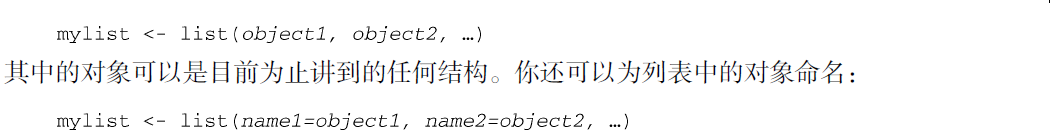
\includegraphics[width=\textwidth]{screenshot003}
\end{figure}

\section{数据的输入}
\begin{figure}[H]
	\centering
	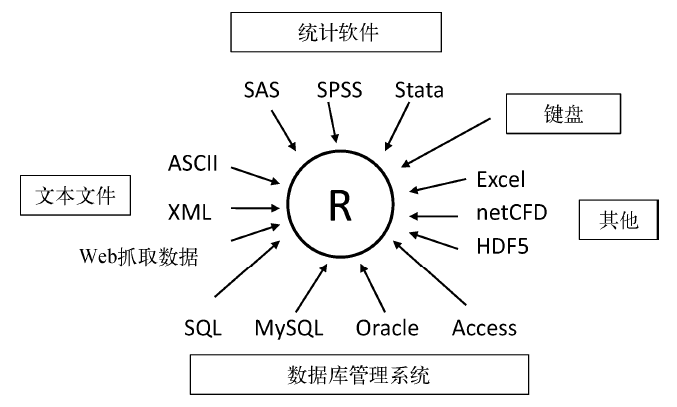
\includegraphics[width=0.6\textwidth]{screenshot004}
	\caption{可供R导入的数据源}
	\label{fig:screenshot004}
\end{figure}

R中的函数edit()会自动调用一个允许手动输入数据的文本编辑器。
\begin{lstlisting}[language=R]
> iris2 <- edit(iris)
\end{lstlisting}

\section{数据集的标注}
\subsection{值标签}
\begin{figure}[H]
	\centering
	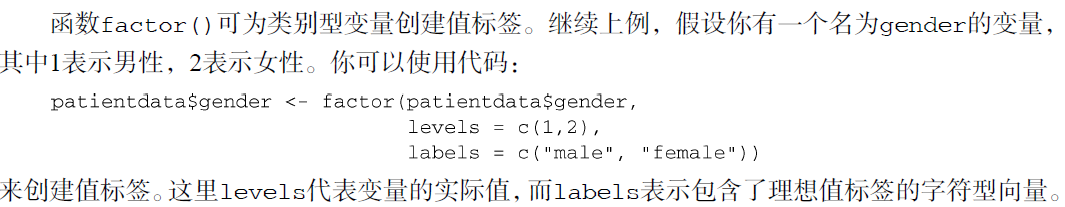
\includegraphics[width=\textwidth]{screenshot005}
\end{figure}

\section{处理数据对象的实用函数}
\begin{figure}[H]
	\centering
	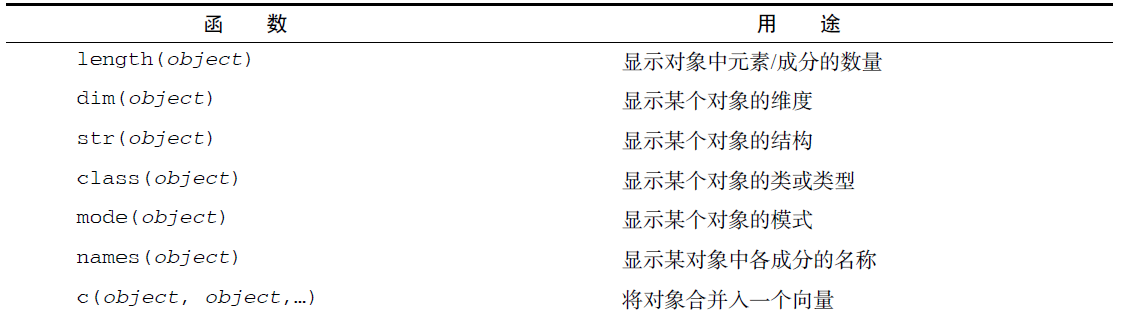
\includegraphics[width=\textwidth]{screenshot006}
\end{figure}
\begin{figure}[H]
	\centering
	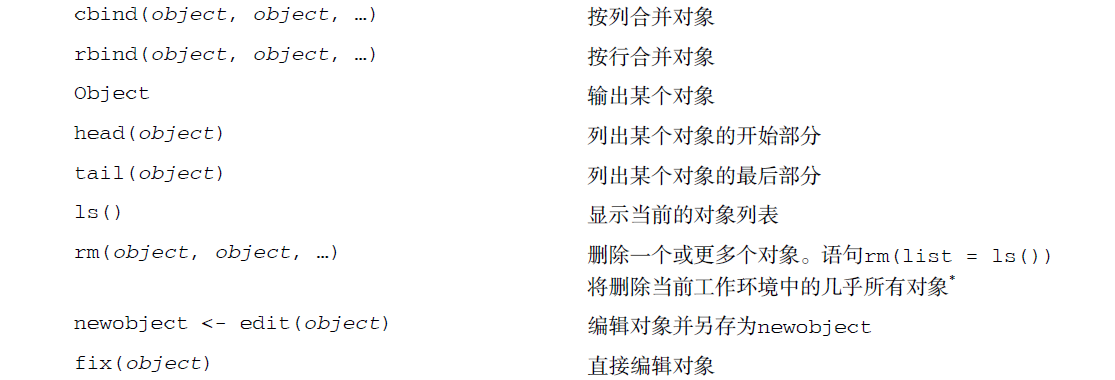
\includegraphics[width=\textwidth]{screenshot007}
\end{figure}

\begin{lstlisting}[language=R]
	
\end{lstlisting}

\begin{lstlisting}[language=R]
	
\end{lstlisting}

\begin{lstlisting}[language=R]
	
\end{lstlisting}

\begin{lstlisting}[language=R]
	
\end{lstlisting}

\begin{lstlisting}[language=R]
	
\end{lstlisting}

\begin{lstlisting}[language=R]
	
\end{lstlisting}

\begin{lstlisting}[language=R]
	
\end{lstlisting}

\begin{lstlisting}[language=R]
	
\end{lstlisting}

\begin{lstlisting}[language=R]
	
\end{lstlisting}

\begin{lstlisting}[language=R]
	
\end{lstlisting}

\begin{lstlisting}[language=R]
	
\end{lstlisting}

\begin{lstlisting}[language=R]
	
\end{lstlisting}

\end{document}